After establishing a theoretical foundation both about multigrid methods and evolutionary grammar-based optimization techniques, the first primary goal of this thesis is to develop a formal language for expressing arbitrarily structured multigrid solvers in a generalized way.
For this purpose, first observe that the multigrid solvers described Section~\ref{sec:multigrid-cycles} can be all classified by their \emph{cycle type}.
Each such cycle possesses a distinct computational pattern which stems from the number of recursive descents performed on each level of the method.
For instance a V-cycle is characterized by exactly one recursive descent per level.
All these classically considered multigrid cycles employ a fixed uniform number of recursive descents and smoothing steps per discretization level, which is determined by the parameters $\gamma$, $\nu_1$ and $\nu_2$ in Algorithm~\ref{alg:multigrid-cycle}.
While the representation of a multigrid method as a recursive cycle yields a formally simple and easily parameterizable algorithmic formulation it also enforces unnecessary restrictions on its structure.
Consider for instance the multigrid method depicted in Figure~\ref{fig:non-traditional-multigrid-cycle}.
\begin{figure}
	\begin{subfigure}{0.1\textwidth}
		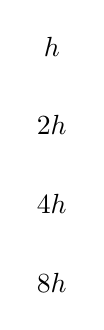
\begin{tikzpicture}
			\node   (h) at (-0.75, 4){$h$};
			\node   (2h) at (-0.75, 3){$2h$};
			\node   (4h) at (-0.75, 2){$4h$};
			\node   (8h) at (-0.75, 1){$8h$};
		\end{tikzpicture}
	\end{subfigure}
	\begin{subfigure}{0.9\textwidth}
		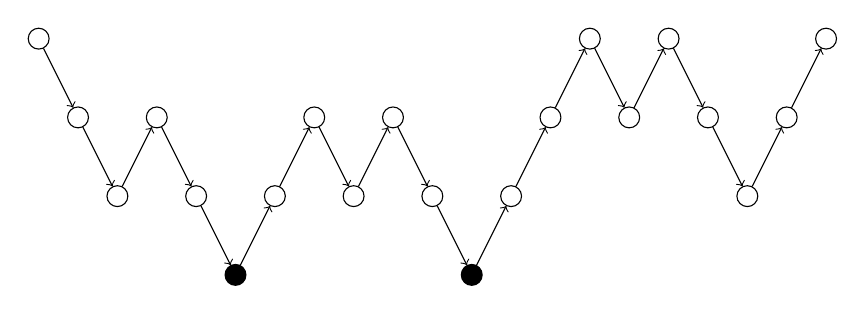
\begin{tikzpicture}
			\node	(a) at (0,4) [draw, circle,scale=0.8] {};
			\node	(b) at (0.5,3) [draw, circle,scale=0.8] {};
			\node	(c) at (1,2) [draw, circle,scale=0.8] {};
			\node	(d) at (1.5,3) [draw, circle, scale=0.8] {};
			\node	(e) at (2,2) [draw, circle, scale=0.8] {};
			\node	(f) at (2.5,1) [draw, circle,scale=0.8,fill=black] {};
			\node	(g) at (3,2) [draw, circle,scale=0.8] {};
			\node	(h) at (3.5,3) [draw, circle,scale=0.8] {};
			\node	(i) at (4,2) [draw, circle,scale=0.8] {};
			\node	(j) at (4.5,3) [draw, circle,scale=0.8] {};
			\node	(k) at (5,2) [draw, circle,scale=0.8] {};
			\node	(l) at (5.5,1) [draw, circle,scale=0.8,fill=black] {};
			\node	(m) at (6,2) [draw, circle,scale=0.8] {};
			\node	(n) at (6.5,3) [draw, circle,scale=0.8] {};
			\node	(o) at (7,4) [draw, circle,scale=0.8] {};
			\node	(p) at (7.5,3) [draw, circle,scale=0.8] {};
			\node	(q) at (8,4) [draw, circle,scale=0.8] {};
			\node	(r) at (8.5,3) [draw, circle,scale=0.8] {};
			\node	(s) at (9,2) [draw, circle,scale=0.8] {};
			\node	(t) at (9.5,3) [draw, circle,scale=0.8] {};
			\node	(u) at (10,4) [draw, circle,scale=0.8] {};
			\draw 
			(a) edge[->] (b) 
			(b) edge[->] (c)
			(c) edge[->] (d)
			(d) edge[->] (e)   
			(e) edge[->] (f)
			(f) edge[->] (g)
			(g) edge[->] (h)
			(h) edge[->] (i)
			(i) edge[->] (j)
			(j) edge[->] (k)
			(k) edge[->] (l)
			(l) edge[->] (m)
			(m) edge[->] (n)
			(n) edge[->] (o)
			(o) edge[->] (p)
			(p) edge[->] (q)
			(q) edge[->] (r)
			(r) edge[->] (s)
			(s) edge[->] (t)
			(t) edge[->] (u)
			;
		\end{tikzpicture}
	\end{subfigure}
	\caption{Example for a non-traditional multigrid method.}
	\label{fig:non-traditional-multigrid-cycle}
\end{figure}
While this method reaches the coarsest level twice and, hence, at first sight looks similar to a W-cycle, it employs a unique pattern of computations that is completely different from those of any of the traditional multigrid cycles.
As a consequence, this method can not be represented within the classical framework of multigrid cycles, as formulated in Algorithm~\ref{alg:multigrid-cycle}.
To overcome these limitations and construct multgrid methods with an arbitrary sequence of computations on each discretization level, as illustrated by the example in Figure~\ref{fig:non-traditional-multigrid-cycle}, a new formal language for their representation is needed.
The first step towards the development of this language is to find a way to represent the current state within each step of a multigrid method and then define transition rules between those states.

\section{Multigrid States}
\label{}
In order to determine how the state of a multigrid method can be represented, we need to reconsider our original formulation of a multigrid cycle in Algorithm~\ref{alg:multigrid-cycle}.
The sake of simplicity, in the following we write symbols that correspond to vectors also in regular font.
In case the mathematical interpretation of a certain lower case symbol is ambiguous, its meaning will be explicitly stated. 
On each level $l > 0$ only the following three operations are employed within a multgrid cycle.
\begin{description}
	\item[Smoothing:] Reduce the oscillatory error components of the approximate solution $\tilde{x}_h$ on the current level. 
	\begin{equation*}
		\tilde{x}_h = \tilde{x}_h + \omega M_h^{-1} \left( b_h - A_h \tilde{x}_h \right) \; \text{where} \; A_h = M_h + N_h
	\end{equation*}
	\item[Restriction:] Restrict the residual to obtain the right-hand side $b_{2h}$ of the error equation on the next coarser level.
	\begin{align*}
		\tilde{x}_{2h} & = 0 \\
 		b_{2h} & = I_h^{2h} (b_h - A_h \tilde{x}_h)
	\end{align*}
	\item[Coarse-Grid Correction:] Prolongate a correction $\tilde{x}_{2h}$ obtained on a coarser grid to reduce the low-frequency error components of the approximate solution $\tilde{x}_h$.
	\begin{equation*}
		\tilde{x}_h = \tilde{x}_h + I_{2h}^h \tilde{x}_{2h}
	\end{equation*}
\end{description}
Now note that except for the operators $A_h$, $I_h^{2h}$ and $I_{2h}^h$ the result of each of these operations exclusively depends on the current value of the approximate solution on subsequent levels, i.e. $\tilde{x}_{h}$ and $\tilde{x}_{2h}$, and the right-hand side $b_h$.
However, in contrast to coarse-grid correction which utilizes the current approximate solution on the coarse grid, both smoothing and restriction first compute the residual $r_h = b_h - A_h \tilde{x}_h$, which can be considered as an intermediate step.
While this differentiation is not strictly necessary it leads to simpler operations, since both restriction and smoothing can then be split into two steps.
Furthermore, as in practice the actual error can usually not be computed, the residual is often the only available metric to investigate whether a multigrid iteration has achieved a certain amount of error reduction and, hence, has to be repeatedly computed.
%The residual is then either restricted and assigned to the right-hand side $b_{2h}$ or employed to reduce the oscillatory error components of the approximate solution by computing a correction term of the form $\omega A_h^{-1} r_h$.
To derive a general representation for the state of a multigrid method based on our previous observations, we consider the sequence of operations shown in Algorithm~\ref{alg:example-three-grid-method}, which corresponds to a three-grid V-cycle that performs one step of underrelaxed Jacobi smoothing on the second finest level.
\begin{algorithm}
	\begin{algorithmic}[1]
		\State $\tilde{x}_{h} = x_{h}^0$
		\State $r_{h} = b_{h} - A_h \tilde{x}_{h} $
		\State $ \tilde{x}_{2h} = 0$
		\State $ b_{2h} = I_{h}^{2h} r_{h}$
		\State $ r_{2h} = b_{2h} - A_{2h} \tilde{x}_{2h}$
		\State $ \tilde{x}_{2h} = \tilde{x}_{2h} + I_{4h}^{2h} A_{4h}^{-1} I_{2h}^{4h} r_{2h}$
		\State $ r_{2h} = b_{2h} - A_{2h} \tilde{x}_{2h}$
		\State $ \tilde{x}_{2h} = \tilde{x}_{2h} + 0.6 \cdot D_{2h}^{-1} r_{2h}$
		\State $\tilde{x}_{h} = \tilde{x}_{h}  + I_{2h}^h \tilde{x}_{2h}$
	\end{algorithmic}
\caption{Example for a three-grid V-cycle}
\label{alg:example-three-grid-method}
\end{algorithm}
In each step of this sequence of operations either the approximate solution, right-hand side or residual is updated on a certain level.
While in practice each of these variables corresponds to a data structure encompassing numerical values, our goal is to represent the algorithmic structure of a multigrid solver in the form of symbolic expressions.
In this case the value of each variable is determined by the expression that computes its value.
Updating a variable, therefore, corresponds to assigning a new expression to the corresponding symbol.
For this purpose, we consider the tuple
\begin{equation*}
	S_h = (\tilde{x}_h, b_h, r_h)
\end{equation*} 
on each level with step size $h$, which then contains expression of each of the corresponding three variables.
Starting from the first line we can then progressively update the contents of this tuple with the expression contained in each line, whereby the occurrence of each symbol is replaced by the respective expression currently contained in the tuple.
Figure~\ref{fig:example-tree-grid-method-states} shows the respective state tuple for each line of Algorithm~\ref{alg:example-three-grid-method}.
\begin{figure}
	\begin{equation*}
		\begin{array}{l l l}
			\hline
			\bm{S_h} & \bm{=} & \bm{(\tilde{x}_h, \, b_h, \, r_h)}  \\
			1: & &  x_{h}^0, \, b_h, \, \lambda \\
			2: & &  x_{h}^0, \, b_h, \, b_{h} - A_h x_{h}^0 \\ \hline
			\bm{S_{2h}} & \bm{=} &  \bm{(\tilde{x}_{2h}, \, b_{2h}, \, r_{2h})} \\
			3: & &  0, \, \lambda, \, \lambda \\
			4: & &  0, \, I_{h}^{2h}\underbrace{(b_{h} - A_h x_{h}^0)}_{r_{h}}, \, \lambda \\
			5: & &  0, \, I_{h}^{2h}(b_{h} - A_h x_{h}^0), \,\underbrace{I_{h}^{2h}(b_{h} - A_h x_{h}^0)}_{b_{2h}} - A_{2h} 0 \\
			6: & & 0 + I_{4h}^{2h} A_{4h}^{-1} I_{2h}^{4h} (\underbrace{I_{h}^{2h}(b_{h} - A_h x_{h}^0) - A_{2h} 0}_{r_{2h}}), \, I_{h}^{2h}(b_{h} - A_h x_{h}^0), \, \lambda\\
			7: & & 0 + I_{4h}^{2h} A_{4h}^{-1} I_{2h}^{4h} (I_{h}^{2h}(b_{h} - A_h x_{h}^0) - A_{2h} 0), \, I_{h}^{2h}(b_{h} - A_h x_{h}^0), \\ 
			& &  \underbrace{I_{h}^{2h}(b_{h} - A_h x_{h}^0)}_{b_{2h}} - A_{2h} (\underbrace{0 + I_{4h}^{2h} A_{4h}^{-1} I_{2h}^{4h} (I_{h}^{2h}(b_{h} - A_h x_{h}^0) - A_{2h} 0)}_{\tilde{u}_{2h}}) \\
			8: & &   (\underbrace{0 + I_{4h}^{2h} A_{4h}^{-1} I_{2h}^{4h} (I_{h}^{2h}(b_{h} - A_h x_{h}^0) - A_{2h} 0)}_{\tilde{u}_{2h}}) + 0.6 \cdot D_{2h}^{-1} \cdot \\ 
			& & (\underbrace{I_{h}^{2h}(b_{h} - A_h x_{h}^0) - A_{2h} (0 + I_{4h}^{2h} A_{4h}^{-1} I_{2h}^{4h} (I_{h}^{2h}(b_{h} - A_h x_{h}^0) - A_{2h} 0))}_{r_{2h}}), \\ 
			& & I_{h}^{2h}(b_{h} - A_h x_{h}^0), \, \lambda \\ \hline 
			\bm{S_h} & \bm{=} & \bm{(\tilde{x}_h, \, b_h, \, r_h)}  \\
			9: & & x_{h}^0 + I_{2h}^h ((0 + I_{4h}^{2h} A_{4h}^{-1} I_{2h}^{4h} (I_{h}^{2h}(b_{h} - A_h x_{h}^0) - A_{2h} 0)) + 0.6 \cdot D_{2h}^{-1} \cdot \\ 
			& &  (I_{h}^{2h}(b_{h} - A_h x_{h}^0) - A_{2h} (0 + I_{4h}^{2h} A_{4h}^{-1} I_{2h}^{4h} (I_{h}^{2h}(b_{h} - A_h x_{h}^0) - A_{2h} 0)))), \\ 
			& &  b_h, \, \lambda \\
			\hline
		\end{array}
	\end{equation*}
	\caption{State tuple in each step of Algorithm~\ref{alg:example-three-grid-method}.}
	\label{fig:example-tree-grid-method-states}
\end{figure}
As it has been introduced in Section~\ref{sec:formal-languages}, the empty symbol $\lambda$ denotes that a certain component of the tuple is unspecified.
After the last step of the sequence (line 9) the first component of the tuple ($\tilde{x}_h$) then combines all computational steps of the method in a single expression.

While Figure~\ref{fig:example-tree-grid-method-states} illustrates that the ternary tuple contains all relevant information of a multigrid method's current state on a certain level, we have not yet considered how to transition between the states of two subsequent levels.
First, consider the case of transitioning from a certain level with step size $h$ to the next coarser level with step size $2h$, which is shown in line 3 and 4 of Figure~\ref{fig:example-tree-grid-method-states}.
Here the tuple
\begin{equation*}
	S_{2h} = (0, \, I_{h}^{2h}(b_{h} - A_h x_{h}^0), \, \lambda)
\end{equation*} 
corresponds to the coarse-grid error equation 
\begin{equation*}
	A_{2h} x_{2h} = I_{h}^{2h}(b_{h} - A_h x_{h}^0),
\end{equation*}
whose solution is to be approximated starting with an initial guess of zero.
Therefore, all information to create this state is obtained from the next finer level in form of the restricted residual $I_h^{2h} r_h = I_h^{2h} (b_{h} - A_h x_{h}^0)$.
On the other hand, consider the transition from a coarse grid back to the next finer grid in form of the coarse-grid correction in line 9.
In this case we both require the approximate solution $\tilde{x}_{2h}$, computed on the coarse grid, as well as the previous values of the first two components $\tilde{x}_h$ and $b_h$ of the fine-grid state tuple.
While in the case of restriction we can neglect all previous states represented on the coarser grid, as it is explicitly contained in the residual, for a coarse-grid correction the previous state on the fine-grid needs to be restored.
Note that in case of a multigrid method that operates on a hierarchy of discretizations of even larger depth than the example shown in Algorithm~\ref{alg:example-three-grid-method}, this process must be recursively performed for each bottom up transition within the hierarchy.
To resolve this issue we need to extend our original formulation of a multgrid state by a fourth component with the purpose of preserving current state of the next finer level.
While at the topmost level this component is always empty, whenever restriction is performed the state of the current level is included.
For instance in line 4 of Figure~\ref{fig:example-tree-grid-method-states} we have to extend the given ternary tuple 
\begin{equation*}
S_{2h} = (0, \, I_{h}^{2h}(b_{h} - A_h x_{h}^0), \, \lambda)
\end{equation*}
by including the state 
\begin{equation*}
S_h = (x_{h}^0, \, b_h, \, b_{h} - A_h x_{h}^0, \, \lambda) 
\end{equation*} 
as an additional fourth entry. 
Hence, all required information for restoring the previous fine-grid state values is then included in the quaternary tuple 
\begin{equation*}
	S_{2h} = (0, \, I_{h}^{2h}(b_{h} - A_h x_{h}^0), \, \lambda, \, S_h).
\end{equation*}
%TODO clarify that line 3 and 4 can in practice be combined to one step
Note that since $S_h$ represents the current state on the finest grid, its fourth component is empty, while otherwise it would refer to the previous state of the next higher level in the discretization hierarchy.
To assess the feasibility of this approach, we have to check whether all components required to construct the coarse-grid correction expression, as in line 9 of Figure~\ref{fig:example-tree-grid-method-states}, are available within the current state.
However, since in addition to $\tilde{x}_{2h}$, both the approximate solution $\tilde{x}_h$ and right-hand side $b_h$ are now contained in the fourth component of the coarse-grid state tuple, this expression can be assembled in a straightforward manner.
At this point, it should be noted that coarse-grid correction from the coarsest grid represents a special case. 
Since the only allowed operation on this level is the application of the coarse-grid solver, which is denoted by a multiplication with the inverse of the system matrix, it is represented as a single operation in form of the expression 
\begin{equation*}
	\tilde{x}_{2h} = \tilde{x}_{2h} + I_{4h}^{2h} A_{4h}^{-1} I_{2h}^{4h} r_{2h}.
\end{equation*}
After resolving the issue of restoring previous states during coarse-grid correction, we can, thus, now provide a complete formal definition of the state of a multigrid method.
\begin{definition}[Multigrid State]
\label{def:multigrid-state}
The state of a multigrid method for solving the equation $A_{2h} x_{2h} = b_{2h}$ on a certain grid with step size $2h$ is given by the quaternary tuple
\begin{equation*}
	S_{h} = \left( \tilde{x}_{h}, b_{h}, c_{h}, S_{h}\right), 
\end{equation*}
where
\begin{itemize}
	\item $\tilde{x}_{h}$ is a mathematical expression for computing an approximate solution of the above equation,
	\item $b_{h}$ is an expression for computing the right-hand side of the above equation,
	\item $c_{h}$ is a correction term for improving the accuracy of the approximate solution,
	\item $S_{h/2}$ is either the current state on the next finer level with a step size $h/2$ or the empty symbol $\lambda$ in case $h$ represents the topmost level in the given hierarchy of discretizations.
\end{itemize}
\end{definition}
Note that in Definition~\ref{def:multigrid-state} the third component $c_{2h}$ of a multigrid state no longer only refers to the residual, but now represents an expression that corresponds to a general correction term.
While in the classical multigrid formulation, as presented in Section~\ref{sec:multigrid-methods}, all smoothing expressions are directly derived from the residual, alternative relaxation methods which can not be easily formulated in the simple framework of stationary iterative methods, such as distributive smoothing, have been proposed~\cite{trottenberg2000multigrid}.
Furthermore, the general notion of a correction term enables us to also represent intermediate expressions that do not specifically refer to the current residual within a multigrid state, for instance $c_h = \omega M_h^{-1} \left( b_h - A_h \tilde{x}_h \right)$ which corresponds to the complete term that is added to the current approximate solution within smoothing.   
%Finally, note that the computation of the coarse-grid correction does not require the value of the previous fine-grid residual.
%Therefore, the corresponding expression does not need to be restored and the residual can be omitted in the respective state tuple when performing the fine-to-coarse grid transition.
\section{State Transition Rules}
After defining the state of a multigrid method, the next step towards developing a formal language for representing arbitrary sequences of multigrid operations,
such as the one shown in Figure~\ref{fig:non-traditional-multigrid-cycle}, is to formally define a set of rules that describes the transitions between all possible states.
For this purpose, we need to consider the set of possible operations within a multigrid method, as described at the beginning of the last section.
From a mathematical point of view, these operations exclusively consist of either matrix-vector multiplications or vector additions and subtractions.
First of all, the computation of the residual $r_h = b_h - A_h \tilde{x}_h$ represents the fundamental operation based on which an approximation to the solution of the target system $A_h x_h = b_h$ is iteratively improved, either with means of smoothing or by computing a coarse-grid correction.
The \textsc{residual} function implements the corresponding state transition for computing the residual on a certain level with step size $h$.
For this purpose first the residual expression is assembled based on the system matrix $A_h$ and the given state $S_h = (\tilde{x}_h, b_h, \lambda, S_{h/2})$, which contains the current approximate solution $\tilde{x}_h$ and right-hand side $b_h$.
The resulting expression is included as a the correction term $c_h$ into $S_h$, which is then returned at the end of the function.
%TODO describe residual
%TODO include references to functions
\begin{algorithm}
	\begin{algorithmic}
		\Function{residual}{$A_h$, $(\tilde{x}_h, b_h, \lambda, S_{h/2})$}
		\State $c_h \gets b_h - A_h \tilde{x}_h$
		\State return $(\tilde{x}_h, b_h, c_h, S_{h/2})$
		\EndFunction
	\end{algorithmic}
\label{alg:state-transition-residual}
\end{algorithm}
After constructing an initial correction $c_h$ from the residual expression $b_h - A_h \tilde{x}_h$, next we can apply an operator $B_h$ to this term, either as part of a smoothing expression or in form of restriction to obtain the right-hand side $b_h$ of the coarse-grid error equation.
Since both operations can be formulated as a matrix-vector multiplication, we consider this operator application as an intermediate step that is implemented in form of the function \textsc{apply}.
This function applies to operator $B_h$ to the current correction term. 
The resulting expression then serves as a new correction term within the returned state.
\begin{algorithm}
	\begin{algorithmic}
		\Function{apply}{$B_h$, $(\tilde{x}_h, b_h, c_h, S_h)$}
		\State return $(\tilde{x}_h, b_h, B_h\cdot c_h, S_h)$
		\EndFunction
	\end{algorithmic}
\end{algorithm}
In general, the choice of the operator $B_h$ corresponds to the two elementary options available within a multigrid method, i.e. smoothing and solving the given problem on a coarser grid.
For instance, the choice of $B_h = D_h^{-1}$ leads to the expression
\begin{equation*}
	c_h = D_{-1} (b_h - A_h \tilde{x}_h),
\end{equation*}
which corresponds to one step of the Jacobi method as shown in Equation~\ref{eq:jacobi-method}.
In contrast, choosing $B_h$ as the restriction operator $I_h^{2h}$ leads to
\begin{equation*}
	c_{2h} = I_{h}^{2h} (b_h - A_h \tilde{x}_h),
\end{equation*}
which then serves as a right-hand side $b_{2h}$ of the corresponding coarse-grid error equation.
In both cases the correction term obtained from the \textsc{apply} function serves a different purpose.
First of all, we must be able to generate an expression that computes an improved approximate solution $\tilde{x}_h$ by applying an update in form of the correction term $c_h$ to the previous value of $\tilde{x}_h$. 
This behavior is implemented in the function \textsc{iterate}, which returns a state tuple with the expression for computing an updated approximate solution as its first entry.
In addition to the sole application of correction term, this function also includes a relaxation factor $\omega$ and partitioning operator $P$ which enables both the formulation of underrelaxed, overrelaxed and potentially colored versions of each operation, for instance those described in Section~\ref{sec:rb-gs}.
\begin{algorithm}
	\begin{algorithmic}
		\Function{cgc}{$I_{2h}^{h}$, ($\tilde{x}_{2h}$, $b_{2h}$, $\lambda$, $S_{h}$)}
		\State ($\tilde{x}_h$, $f_{h}$, $c_h$, $S_{h/2}$) $\gets S_{h}$
		\State $c_h \gets I_{2h}^{h} \cdot \tilde{x}_{2h}$
		\State return ($\tilde{x}_h$, $f_{h}$, $c_h$, $S_{h/2}$)
		\EndFunction
	\end{algorithmic}
\end{algorithm}
%TODO describe partitioning and relaxation factor
%TODO describe cocy first! Then cgc

As described in the last section, coarse-grid correction (\textsc{cgc}) comprises an additional preliminary step in which the previous state on the next higher level is restored.
After constructing a correction term, we next need to define a state transition that corresponds to the application of this correction to the current approximate solution in order to further improve its accuracy.
Again, we formulate this transition as a function of the following form.
\begin{algorithm}
\begin{algorithmic}
	\Function{iterate}{$\omega$, $P$, ($\tilde{x}_h$, $b_h$, $c_h$, $S_{h/2}$)}
	\State $\tilde{x}_h \gets \tilde{x}_h + \omega \cdot c_h$ with $P$
	\State return ($\tilde{x}_h$, $b_h$, $\lambda$, $S_{h/2}$) 
	\EndFunction
\end{algorithmic}
\end{algorithm}
%TODO describe restriction
\begin{algorithm}
	\begin{algorithmic}
		\Function{cocy}{$A_{2h}$, $x_{2h}^0$, ($\tilde{x}_h$, $b_{h}$, $c_{2h}$, $S_{h/2}$)}
		\State $\tilde{x}_{2h} \gets x_{2h}^0$ 
		\State $b_{2h} \gets c_{2h}$
		\State $c_{2h} \gets b_{2h} - A_{2h} \tilde{x}_{2h}$ 
		\State $S_h \gets$ ($\tilde{x}_{2h}$, $b_{h}$, $\lambda$, $S_{h/2}$)
		\State return ($\tilde{x}_{2h}$, $b_{2h}$, $c_{2h}$, $S_h$)
		\EndFunction
	\end{algorithmic}
\end{algorithm}

